\chapter{Implementasi dan Pengujian Prototipe}

Bab Implementasi dan Pengujian Prototipe berisi tentang lanjutan dari metodologi \textit{User-Centered Design}, yaitu tahap perancangan serta evaluasi prototipe desain solusi. Kedua tahap tersebut dilakukan iterasi dengan jumlah sesuai kebutuhan. Perancangan dan evaluasi akan dilakukan pada \textit{low-fidelity prototype} berbentuk \textit{wireframe} dan \textit{high-fidelity prototype} berbentuk prototipe \textit{mobile application} pada perangkat Android. Bagian perancangan prototipe menjelaskan tentang proses implementasi dari prototipe, sedangkan bagian evaluasi akan menjelaskan tentang proses pengujian prototipe yang berisi skenario dan hasil pengujian yang telah dicocokan dengan \textit{usability goals} dan \textit{user experience goals} yang sudah ditentukan sebelumnya. 


% * =======================================================================
% *   ||  ||  ||  ||  ||  ||  ||  ||  ||  ||  ||  ||  ||  ||  ||  ||  ||
% * =======================================================================

\section{Pengembangan Prototipe \textit{Low-Fidelity}}
\label{sec:lofi}

Prototipe \textit{Low-Fidelity} adalah sebuah cara yang efektif untuk merealisasi rancangan solusi dari sebuah desain beserta dengan konsep-konsep desain menjadi sebuah artefak yang dapat dilakukan interaksi oleh pengguna produknya. \parencite{adobe2017prototype} Tujuan dari pembuatan prototipe \textit{low-fidelity} adalah untuk merealisasikan fungsionalitas inti dari produk sehingga tersampaikan kepada pengguna, sebelum mengikutsertakan elemen-elemen visual lainnya. 

\newpage

\subsection{Perancangan Navigasi Prototipe}
\label{subsec:lofi_navigasi}
Perlu dibentuk rancangan navigasi yang akan menghubungkan halaman-halaman yang telah ditentukan pada Tabel \ref{tab:daftar_halaman}. Pada Gambar \ref{fig:diagram_navigasi} dapat ditemukan Diagram Navigasi yang menggambarkan hubungan interaksi antarhalaman dari prototipe. Hal ini akan menjadi salah satu dari acuan pengujian prototipe \textit{low-fidelity}.
Perlu diingat bahwa widget akan diimplementasikan dalam prototipe, namun widget tidak dapat diakses langsung dari aplikasi melainkan perlu ditambahkan ke dalam Homescreen dari \textit{smartphone}, sehingga widget tidak termasuk ke dalam Diagram Navigasi.  

\newpage

\begin{landscape}
  \begin{figure}[h]
    \centering
    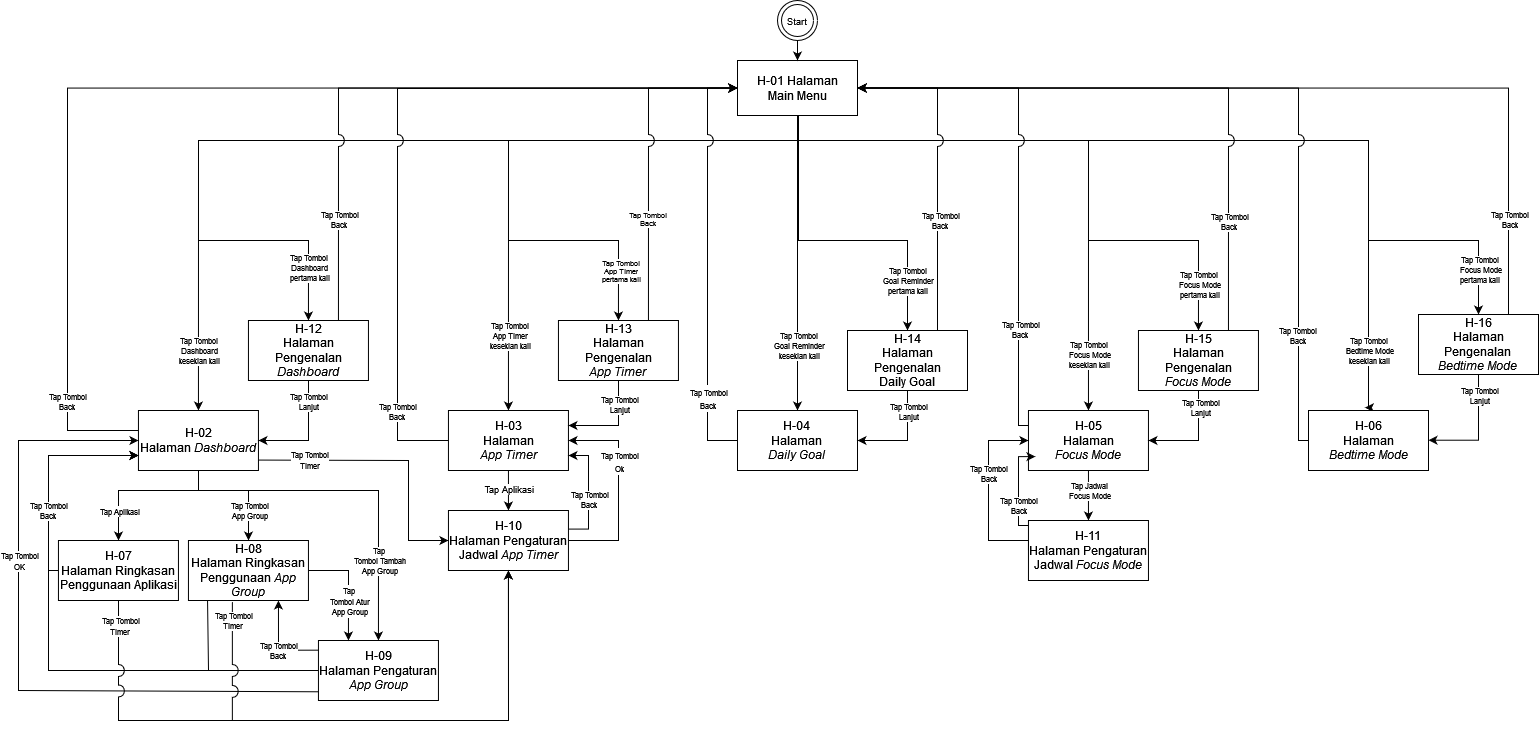
\includegraphics[width=1.7\textwidth]{chapter-4-diagram-navigasi.png}
    \caption{Diagram Navigasi}
    \label{fig:diagram_navigasi}
  \end{figure}
\end{landscape}

\newpage


\subsection{Implementasi Prototipe \textit{Low-Fidelity}}
\label{subsec:lofi_implementasi}
Tampilan dari halaman serta widget yang telah ditentukan perlu memuat informasi dan elemen interaksi yang cukup bagi pengguna untuk mencapai tujuannya saat menggunakan prototipe \textit{low-fidelity}. Tabel \ref{tab:daftar_lofi_halaman} memuat implementasi tampilan halaman prototipe \textit{low-fidelity}, sedangkan Tabel \ref{tab:daftar_lofi_widget} memuat implementasi tampilan untuk widget. Pada kedua tabel tersebut dimuat juga pemetaan beberapa prinsip desain yang telah disebutkan pada Tabel \ref{tab:prinsip_desain} terhadap prototipe \textit{low-fidelity}, serta penjelasan singkat tentang tampilan.

\newpage


\newlength{\lofiwidth}
\setlength{\lofiwidth}{0.325\textwidth}


\newlength{\lofidescwidth}
\setlength{\lofidescwidth}{0.35\textwidth}

\newcommand{\desc}[2]{\begin{minipage}[t]{#1}\linespread{1.0}\selectfont{#2}\end{minipage}}
\newcommand{\lofidesc}[1]{\desc{\lofidescwidth}{#1}}

\newcommand{\lofi}[1]{\begin{center}\includegraphics[width=\lofiwidth]{#1}\end{center}}
\newcommand{\lofiwidget}[2]{\begin{center}\includegraphics[width=#1]{#2}\end{center}}

\RaggedLeft
\begin{footnotesize}
\begin{longtable}[c]{|>{\ccnormspacingcenter}p{0.12\textwidth}|>{\ccnormspacing}p{\lofidescwidth}|>{\ccnormspacingcenter}p{0.1\textwidth}|>{\ccnormspacingcenter}p{\lofiwidth}|}
  \caption{Daftar Tampilan Halaman Prototipe \textit{Low-Fidelity}}
  \label{tab:daftar_lofi_halaman} \\
  \hline \rowcolor[HTML]{A3E5F5}
  \centering\textbf{Halaman} & \centering\textbf{Penjelasan Halaman} & \centering\textbf{Prinsip Desain} & \textbf{Prototipe \textit{Low-Fidelity}} \\ \hline \endfirsthead
  \hline \rowcolor[HTML]{A3E5F5}
  \centering\textbf{Halaman} & \centering\textbf{Penjelasan Halaman} & \centering\textbf{Prinsip Desain} & \textbf{Prototipe \textit{Low-Fidelity}} \\ \hline \endhead
  \hline \endfoot

  \textbf{H-01} Halaman Main Menu & 
    \lofidesc{
      Halaman ini adalah tampilan utama dari aplikasi Digital Wellbeing yang memuat navigasi utama ke fitur-fitur seperti Dashboard, App Timer, Daily Goal, Focus Mode, dan Bedtime Mode. Navigasi menuju Dashboard diletakkan di paling atas beserta \textit{pie graph} yang menunjukkan aktivitas \textit{smartphone} pengguna di hari tersebut. Di bagian bawah juga terdapat navigasi menuju pengaturan notifikasi dan mode "Do Not Disturb" bawaan \textit{smartphone}
    } & DP-01, DP-02, DP-04, DP-05, DP-08, DP-09 & \lofi{lofi/h-01} \\ \hline

  \textbf{H-02} Halaman Dashboard & 
  \lofidesc{
    Halaman ini memuat seluruh data penggunaan \textit{smartphone}. Pada bagian paling atas, terdapat rekomendasi dari Digital Wellbeing tentang langkah-langkah yang dapat dilakukan pengguna untuk memperbaiki kebiasaan digitalnya, atau penanda jika kebiasaannya sudah cukup sehat. Bagian rekomendasi ini adalah salah satu aspek di mana tipe interaksi \textit{responding} difokuskan. Data penggunaan \textit{smartphone} yang ditampilkan dapat dipilih oleh menu, baik waktu penggunaan aplikasi, jumlah notifikasi, atau jumlah pembukaan aplikasi. Periode durasi data juga dapat dipilih dengan menu, baik secara per jam, harian, atau mingguan. \newline
    Selain itu terdapat daftar seluruh aplikasi pada \textit{smartphone} beserta data penggunaannya masing-masing. Pengguna dapat melihat data lebih detail atau langsung memasang App Timer. Pengguna juga dapat melihat data penggunaan dari kelompok aplikasi yang telah dibuat, atau membuatnya jika belum ada, terlihat tepat di atas daftar. Jika pengguna ingin mencari aplikasi spesifik, maka \textit{searchbar} bisa dimanfaatkan untuk mengetikkan nama aplikasi.
  } & DP-01, DP-02, DP-03, DP-04, DP-05, DP-08, DP-09 & \lofi{lofi/h-02} \\ \hline

  \textbf{H-03} Halaman App Timer & 
    \lofidesc{
      Halaman ini berisi daftar App Timer yang telah dipasang oleh pengguna, waktu yang telah dilampaui selama menggunakan aplikasi tersebut, serta sisa waktu sebelum aplikasi ditutup aksesnya. Pengguna bisa mengubah pengaturan App Timer yang telah dipasang, atau menambah aplikasi atau App Group yang ingin dipasangkan App Timer dengan mencarinya dari daftar aplikasi yang terletak di bawah. Di halaman ini pengguna juga bisa mengatur perilaku pemberian peringatan terhadap sisa waktu aplikasi-aplikasi.
    } & DP-02, DP-03, DP-05, DP-08, DP-09 & \lofi{lofi/h-03} \\ \hline
  
  \textbf{H-04} Halaman Daily Goal & 
    \lofidesc{
      Di halaman ini, pengguna dapat menentukan Daily Goal atau tujuan harian yang ingin ditempuh dan dibantu diingatkan oleh aplikasi Digital Wellbeing. Pengguna dapat mengatur perilaku pengiriman peringatannya. Pengguna juga dapat menyalakan fitur Smartphone Usage Evaluation di mana aplikasi akan mengirimkan sebuah notifikasi berisi jumlah waktu penggunaan \textit{smartphone} pada hari tersebut serta peringatan untuk mengevaluasi Daily Goal yang telah ditentukan.
    } & DP-03, DP-05, DP-06, DP-08, DP-09 & \lofi{lofi/h-04} \\ \hline
  
  \textbf{H-05} Halaman Focus Mode & 
    \lofidesc{
      Halaman ini memuat status dari keberjalanan Focus Mode serta aksi-aksi yang dapat dilakukan untuk menunda, mematikan, atau mengaktivasinya. Selain itu, terdapat juga daftar jadwal Focus Mode yang ditentukan pengguna, atau pilihan untuk menambahkannya. Jadwal Focus Mode akan menavigasikan pengguna ke halaman pengaturan jadwal tersebut.
    } & DP-03, DP-05, DP-06, DP-08, DP-09 & \lofi{lofi/h-05} \\ \hline
  
  \textbf{H-06} Halaman Bedtime Mode & 
    \lofidesc{
      Pada halaman ini, pengguna dapat mengatur jadwal aktivasi Bedtime Mode menurut mode perilaku aktivasi yang dipilihnya. Pengguna juga dapat mengatur kemampuan apa saja yang akan aktif jika Bedtime Mode berlangsung.
    } & DP-03, DP-04, DP-05, DP-08, DP-09 & \lofi{lofi/h-06-schedule} \\ \hline
  
  \textbf{H-07} Halaman Ringkasan Penggunaan Aplikasi & 
    \lofidesc{
      Halaman ini memuat data penggunaan sebuah aplikasi. Jenis data-data yang ditampilkan mirip seperti yang dapat ditemukan pada halaman Dashboard, namun hanya untuk satu buah aplikasi yang dipilih saja. Pemilihan periode waktu serta navigasi waktu data juga dapat dilakukan. Sebagai tambahan, terdapat navigasi ke halaman pengaturan App Timer untuk aplikasinya, serta navigasi menuju halaman pengaturan notifikasi aplikasi bawaan \textit{smartphone}. Tampilan data penggunaan aplikasi sengaja dibuat serupa dengan tampilan pengguna \textit{smartphone} agar pengguna dapat dengan mudah menggunakannya tanpa perlu mempelajari ulang.
    } & DP-05, DP-08, DP-09 & \lofi{lofi/h-07} \\ \hline
  
  \textbf{H-08} Halaman Ringkasan Penggunaan App Group & 
    \lofidesc{
      Halaman ini memuat data penggunaan dari App Group atau kelompok aplikasi yang ditentukan oleh pengguna. Jenis data-data yang ditampilkan mirip seperti yang dapat ditemukan pada halaman Dashboard, namun hanya untuk gabungan dari beberapa aplikasi yang ditentukan. Pemilihan periode waktu serta navigasi waktu data juga dapat dilakukan. Di bagian bawah, terdapat daftar aplikasi yang termasuk ke dalam App Group, yang dapat dinavigasi ke halaman data penggunaan aplikasinya masing-masing, atau halaman pengaturan App Timer aplikasinya. Sebagai tambahan, terdapat juga navigasi ke halaman App Timer untuk App Group tersebut, di mana dapat diatur App Timer untuk keseluruhan aplikasi secara kolektif. Terdapat juga navigasi ke halaman pengaturan App Group jika pengguna ingin melakukan perubahan.
    } & DP-05, DP-08, DP-09 & \lofi{lofi/h-08} \\ \hline
  
  \textbf{H-09} Halaman Pengaturan App Group & 
    \lofidesc{
      Pada halaman ini dapat dilakukan pengaturan terhadap App Group yang dibuat oleh pengguna. Pengaturan App Group termasuk nama App Group serta aplikasi-aplikasi yang dipilih. Pengguna dapat memanfaatkan \textit{searchbar} jika ingin mencari aplikasi yang spesifik.
    } & DP-05, DP-08, DP-09 & \lofi{lofi/h-09} \\ \hline
  
  \textbf{H-10} Halaman Pengaturan Jadwal App Timer & 
    \lofidesc{
      Pada halaman ini dapat dilakukan pengaturan terhadap App Timer aplikasi yang dibuat oleh pengguna. Pengguna dapat mengatur App Timer agar memiliki batas waktu yang sama setiap hari, atau batas waktu yang berbeda-beda per harinya sesuai kebutuhan pengguna. Pengguna juga dapat menghapus App Timer lewat halaman ini. Di bagian atas juga terdapat visualisasi waktu penggunaan aplikasi dan sisa batas waktunya untuk hari tersebut.
    } & DP-01, DP-02, DP-03, DP-05, DP-08, DP-09 & \lofi{lofi/h-10-custom} \\ \hline
  
  \textbf{H-11} Halaman Pengaturan Jadwal Focus Mode & 
    \lofidesc{
      Pada halaman ini, pengguna dapat mengatur hari dan waktu aktivasi dari jadwal Focus Mode yang dibuat pengguna. Pengguna juga dapat mengatur nama dari jadwal, dan aplikasi apa saja yang akan diblokir aksesnya selama jadwal Focus Mode berlangsung. Jika pengguna ingin mencari aplikasi spesifik, maka \textit{searchbar} dapat dimanfaatkan dengan mengetikkan nama aplikasinya.
    } & DP-03, DP-05, DP-08, DP-09 & \lofi{lofi/h-11} \\ \hline
  
  
  \textbf{H-12} Halaman Pengenalan Dashboard & 
    \lofidesc{
      Halaman ini memuat ilustrasi tujuan dari Dashboard dan penjelasan tentang fitur-fitur yang terdapat pada Dashboard. Halaman ini bertujuan agar pengguna memiliki gambaran umum tentang apa yang dapat dicapai dari menggunakan Dashboard.
    } & DP-05, DP-09 & \lofi{lofi/h-12} \\ \hline
  
  \textbf{H-13} Halaman Pengenalan App Timer & 
    \lofidesc{
      Halaman ini memuat ilustrasi tujuan dari App Timer dan penjelasan tentang fitur-fitur yang terdapat pada App Timer. Halaman ini bertujuan agar pengguna memiliki gambaran umum tentang apa yang dapat dicapai dari menggunakan App Timer.
    } & DP-05, DP-09 & \lofi{lofi/h-13} \\ \hline
  
  \textbf{H-14} Halaman Pengenalan Goal Reminder & 
    \lofidesc{
      Halaman ini memuat ilustrasi tujuan dari Daily Goal dan penjelasan tentang fitur-fitur yang terdapat pada Daily Goal. Halaman ini bertujuan agar pengguna memiliki gambaran umum tentang apa yang dapat dicapai dari menggunakan Daily Goal.
    } & DP-05, DP-09 & \lofi{lofi/h-14} \\ \hline
  
  \textbf{H-15} Halaman Pengenalan Focus Mode & 
    \lofidesc{
      Halaman ini memuat ilustrasi tujuan dari Focus Mode dan penjelasan tentang fitur-fitur yang terdapat pada Focus Mode. Halaman ini bertujuan agar pengguna memiliki gambaran umum tentang apa yang dapat dicapai dari menggunakan Focus Mode.
    } & DP-05, DP-09 & \lofi{lofi/h-15} \\ \hline
  
  \textbf{H-16} Halaman Pengenalan Bedtime Mode & 
    \lofidesc{
      Halaman ini memuat ilustrasi tujuan dari Bedtime Mode dan penjelasan tentang fitur-fitur yang terdapat pada Bedtime Mode. Halaman ini bertujuan agar pengguna memiliki gambaran umum tentang apa yang dapat dicapai dari menggunakan Bedtime Mode
    } & DP-05, DP-09 & \lofi{lofi/h-16} \\ \hline


\end{longtable}
\end{footnotesize}
\justifying
\FloatBarrier

\RaggedLeft
\begin{footnotesize}
\begin{longtable}[c]{|>{\ccnormspacingcenter}p{0.1\textwidth}|>{\ccnormspacing}p{0.35\textwidth}|>{\ccnormspacingcenter}p{0.11\textwidth}|>{\ccnormspacingcenter}p{\lofiwidth}|}
  \caption{Daftar Tampilan Widget Prototipe \textit{Low-Fidelity}}
  \label{tab:daftar_lofi_widget} \\
  \hline \rowcolor[HTML]{A3E5F5}
  \centering\textbf{Widget} & \centering\textbf{Penjelasan Widget} & \centering\textbf{Prinsip Desain} & \textbf{Prototipe \textit{Low-Fidelity}} \\ \hline \endfirsthead
  \hline \rowcolor[HTML]{A3E5F5}
  \centering\textbf{Widget} & \centering\textbf{Penjelasan Widget} & \centering\textbf{Prinsip Desain} & \textbf{Prototipe \textit{Low-Fidelity}} \\ \hline \endhead
  \hline \endfoot

  \textbf{W-01} Widget Dashboard & 
    \lofidesc{
      Widget ini memuat data penggunaan \textit{smartphone}, serta 3 aplikasi dengan penggunaan tertinggi pada hari tersebut. Pengguna dapat melakukan navigasi langsung ke halaman Dashboard melalui widget ini.
    } & DP-02, DP-05, DP-09 & \lofiwidget{0.2\textwidth}{lofi/w-01} \\ \hline

  \textbf{W-02} Widget App Timer & 
    \lofidesc{
      Widget ini memuat daftar aplikasi yang telah dipasang App Timer, serta sisa waktu untuk menggunakan aplikasi sebelum aksesnya ditutup. Pengguna dapat melakukan navigasi langsung ke halaman App Timer, atau menambah App Timer untuk aplikasi lain melalui widget ini.
    } & DP-02, DP-05, DP-09 & \lofiwidget{0.3\textwidth}{lofi/w-02} \\ \hline
 
  \textbf{W-03} Widget Focus Mode & 
    \lofidesc{
      Widget ini menampilkan status keberlangsungan dari Focus Mode. Pengguna dapat mengaktivasi Focus Mode langsung dari widget jika sedang tidak aktif, serta mengambil istirahat dan mematikan Focus Mode jika sedang aktif. Pengguna juga dapat melakukan navigasi langsung ke halaman Focus Mode langsung dari widget.
    } & DP-03, DP-04, DP-05, DP-09 & \lofiwidget{0.3\textwidth}{lofi/w-03} \\ \hline

\end{longtable}
\end{footnotesize}
\justifying
\FloatBarrier

% * =======================================================================
% *   ||  ||  ||  ||  ||  ||  ||  ||  ||  ||  ||  ||  ||  ||  ||  ||  ||
% * =======================================================================

\section{Pengujian Prototipe \textit{Low-Fidelity}}
Rancangan prototipe \textit{Low-Fidelity} perlu diuji untuk memastikan bahwa fungsionalitas inti yang telah direalisasikan pada prototipe dapat dipahami pengguna dengan benar, serta memastikan bahwa alur navigasi prototipe sesuai dengan Diagram Navigasi pada Gambar \ref{fig:diagram_navigasi} yang telah dibuat. Pengujian prototipe \textit{low-fidelity} dilakukan untuk mencapai 2 tujuan, yaitu untuk memastikan navigasi dari prototipe sesuai dengan navigasi yang diharapkan oleh desainer menurut Diagram Navigasi pada Gambar \ref{fig:diagram_navigasi}, serta memastikan bahwa informasi yang tertera di prototipe dapat cukup membantu pengguna dalam memenuhi tujuannya. Pengujian ini akan dilakukan kepada lima orang partisipan yang termasuk ke dalam persona primer. Hal ini sesuai dengan perkataan dari \textcite{nielsenusabilityproblems} yang menyebutkan bahwa pengujian dengan 5 orang sudah cukup untuk menemukan rata-rata 85\% masalah dari desain, dalam hal ini dari prototipe \textit{low-fidelity}.


% Pengujian ini akan dilakukan kepada 5 orang pengguna, yang terdiri dari 3 orang yang termasuk ke dalam Persona 2 (Maya) dan 2 orang yang termasuk ke dalam Persona 3 (Nathan). Hal ini sesuai 
% Pengujian belum melibatkan \textit{usability goals} dan \textit{user experience goals} karena terbatasnya elemen-elemen visual dan interaksi yang mendukung dalam mencapai tujuan-tujuan tersebut.

Dalam melakukan pengujian, diperlukan skenario-skenario pengujian berisi \textit{task} yang perlu dilakukan partisipan, serta pertanyaan singkat mengenai pengalaman partisipan dalam mengerjakan \textit{task} tersebut. Skenario pengujian dibuat berdasarkan skenario pengguna yang telah dibahas pada bagian \ref{subsubsec:skenario_pengguna}. Skenario pengujian beserta pemetaannya dengan skenario pengguna dapat ditemukan pada Lampiran \ref{chpt:skenario_lofi}, sedangkan hasil lengkap pengujian dapat ditemukan pada Lampiran \ref{chpt:hasil_test_lofi}.

Dari melakukan pengujian, ditemukan beberapa temuan penting mengenai prototipe \textit{low-fidelity} sehingga perlu dilakukan evaluasi sebelum lanjut ke tahap perancangan prototipe \textit{high-fidelity}. Temuan-temuan penting dari setiap partisipan dapat dilihat pada Tabel \ref{tab:daftar_temuan_lofi}.

\newcommand{\cditem}[1]{\colorbox{white}{\raisebox{7pt}{\begin{minipage}[t]{0.8\textwidth}\linespread{1}\selectfont \begin{itemize}[parsep=0pt, leftmargin=*] #1 \end{itemize} \end{minipage}}}}

\RaggedLeft
\begin{small}
\begin{longtable}[c]{|W{c}{0.12\textwidth}|>{\ccnormspacingcenter}m{0.8\textwidth}|}
  \caption{Daftar Temuan Penting Pengujian Prototipe \textit{Low-Fidelity}}
  \label{tab:daftar_temuan_lofi} \\
  \hline \rowcolor[HTML]{A3E5F5}
  \textbf{Partisipan} & \textbf{Temuan Penting} \\ \hline \endfirsthead
  \hline \rowcolor[HTML]{A3E5F5}
  \textbf{Partisipan} & \textbf{Temuan Penting} \\ \hline \endhead
  \hline \endfoot

  1 & \cditem{
    \item Partisipan merasa alur navigasi cukup mudah untuk diikuti dalam mencapai \textit{task-task} yang dikerjakan
    \item Partisipan merasa widget-widget sangat membantu memudahkan aktivasi fitur-fitur atau melihat data
    \item Partisipan merasa perlu penjelasan lebih tentang kemampuan yang dapat aktif saat Bedtime Mode
    \item Partisipan merasa perlu ada tombol konfirmasi untuk halaman pengaturan App Timer
    \item Partisipan merasa perlu ada suatu \textit{feedback} ketika berhasil menunda App Timer
  } \\ \hline
    
  2 & \cditem{
    \item Partisipan mengerti untuk mengerjakan seluruh \textit{task} yang diberikan saat pengujian 
    \item Partisipan merasa penjelasan pada halaman-halaman pengenalan fitur terlalu kecil dan terlalu panjang
  } \\ \hline
      
  3 & \cditem{
    \item Partisipan merasa navigasi ke halaman penambahan App Group sulit dibedakan dengan navigasi ke halaman penggunaan App Group
    \item Partisipan merasa desain dari radio button membuat sulit untuk membedakan antara pilihan yang dipilih dan tidak
    \item Partisipan merasa fitur "Turn off for now" sebaiknya diganti nama menjadi "Turn off for today"
    \item Partisipan merasa navigasi untuk ke halaman penambahan jadwal Focus Mode sebaiknya dipindah agar mudah diakses jika jadwalnya sudah banyak 
  } \\ \hline
  
  4 & \cditem{
    \item Partisipan merasa widget sangat membantu dan cukup mewakili fungsionalitas utama dari fitur-fiturnya
    \item Partisipan merasa pengaturan untuk pengingat App Timer sedikit sulit untuk dipelajari 
    \item Partisipan merasa perlu ada tombol konfirmasi untuk mengatur App Timer
    \item Partisipan merasa ingin dapat menunda App Timer dari notifikasi pengingat
  } \\ \hline
  
  5 & \cditem{
    \item Partisipan merasa sangat terbantu dengan adanya widget untuk fitur-fitur
    \item Partisipan merasa untuk halaman pengaturan App Timer memerlukan pemilihan App Group yang serupa dengan halaman Dashboard
    \item Partisipan merasa ingin dapat memilih aplikasi yang mendistraksi di luar halaman pengaturan jadwal Focus Mode agar bisa diblokir tanpa jadwal
    \item Partisipan merasa perlu ada opsi untuk mengambil istirahat dengan waktu yang ditentukan sendiri
    \item Partisipan merasa kegunaan pengingat untuk Daily Goal sulit dimengerti dan perlu penjelasan tambahan
    \item Partisipan merasa perlu ada penjelasan singkat tentang mode aktivasi While Charging untuk Bedtime Mode 
  } \\ \hline

\end{longtable}
\end{small}
\justifying
\FloatBarrier

Berdasarkan temuan-temuan yang telah disebutkan di atas, maka disusun beberapa rencana perbaikan terhadap prototipe \textit{low-fidelity}. Rencana perbaikan ini direalisasikan bersamaan dengan perancangan prototipe \textit{high-fidelity} yang dilakukan pada tahap berikutnya. Pada Tabel \ref{tab:daftar_perbaikan_lofi} dapat ditemukan daftar masalah yang disimpulkan dari temuan-temuan penting, beserta rencana perbaikan yang berkaitan.

\RaggedLeft
\begin{small}
\begin{longtable}[c]{|W{c}{0.05\textwidth}|>{\ccnormspacing}m{0.43\textwidth}|>{\ccnormspacing}m{0.43\textwidth}|}
  \caption{Daftar Rencana Perbaikan Prototipe \textit{Low-Fidelity}}
  \label{tab:daftar_perbaikan_lofi} \\
  \hline \rowcolor[HTML]{A3E5F5}
  \textbf{No} & \multicolumn{1}{|c|}{\textbf{Kesimpulan Masalah dari Temuan}} & \multicolumn{1}{|c|}{\textbf{Rencana Perbaikan}} \\ \hline \endfirsthead
  \hline \rowcolor[HTML]{A3E5F5}
  \textbf{No} & \multicolumn{1}{|c|}{\textbf{Kesimpulan Masalah dari Temuan}} & \multicolumn{1}{|c|}{\textbf{Rencana Perbaikan}}\\ \hline \endhead
  \hline \endfoot

  1 & Kurang jelasnya deskripsi untuk fitur-fitur pada Halaman Daily Goal & Menambahkan penjelasan untuk fitur Smartphone Usage Evaluation dan notifikasi pengingat untuk Daily Goal \\ \hline
  2 & Kurangnya penjelasan untuk fitur-fitur di halaman Bedtime Mode & Menambahkan deskripsi singkat untuk pengaturan kemampuan yang dapat aktif saat Bedtime Mode dan mode aktivasi While Charging \\ \hline
  3 & Kurangnya elemen konfirmasi pada pengaturan fitur App Timer & Menambahkan aksi untuk melakukan konfirmasi untuk pengaturan App Timer \\ \hline
  4 & Kurangnya elemen umpan balik ketika berhasil menunda App Timer & Menambahkan pesan umpan balik saat menunda App Timer \\ \hline
  5 & Penjelasan yang sulit dibaca pada halaman-halaman pengenalan fitur & Mengembangkan penjelasan pada halaman-halaman pengenalan dengan memperbesar tulisan dan menambah ilustrasi \\ \hline
  6 & Kurang jelasnya fitur penundaan fitur hanya untuk hari tersebut & Mengubah sususnan kata "Turn off for now" menjadi "Turn off for today" \\ \hline
  7 & Terdapat elemen-elemen navigasi yang berpotensi untuk sulit diraih & Memindahkan elemen navigasi ke posisi yang lebih mudah terlihat \\ \hline
  8 & Sulitnya membedakan opsi yang terpilih untuk pilihan yang menggunakan radio button & Mengubah desain radio button menjadi lebih mudah dipahami \\ \hline
  9 & Kurangnya elemen umpan balik ketika berhasil membuat jadwal Bedtime Mode & Menambahkan pesan umpan balik saat mengatur jadwal Bedtime Mode \\ \hline
  10 & Diperlukannya alur lebih mudah dalam menunda batas waktu App Timer & Menambahkan aksi menunda batas waktu App Timer lewat notifikasi \\ \hline
  11 & Kurang jelasnya kemampuan untuk memilih App Group pada halaman App Timer & Menambahkan bagian khusus pemilihan App Group untuk halaman App Timer \\ \hline
  12 & Kurangnya kemampuan memilih aplikasi mendistraksi umum di luar jadwal & Menambahkan daftar pemilihan aplikasi mendistraksi pada halaman Focus Mode \\ \hline
  
\end{longtable}
\end{small}
\justifying
\FloatBarrier





% * =======================================================================
% *   ||  ||  ||  ||  ||  ||  ||  ||  ||  ||  ||  ||  ||  ||  ||  ||  ||
% * =======================================================================

\newpage


\section{Pengembangan Prototipe \textit{High-Fidelity} Iterasi Pertama}
\label{sec:hifi_1}

Prototipe \textit{high-fidelity} adalah implementasi dari solusi desain yang dibuat sedekat mungkin dengan produk aslinya. Prototipe \textit{high-fidelity} memiliki fungsionalitas, elemen visual, dan interaksi yang lebih lengkap daripada prototipe \textit{low-fidelity} \parencite{PreeceRogersSharp15}. Prototipe yang dirancang mengembangkan seluruh tampilan pada Tabel \ref{tab:daftar_lofi_halaman} dan Tabel \ref{tab:daftar_lofi_widget} di bagian \ref{sec:lofi} pengembangan prototipe \textit{low-fidelity}, serta menerapkan lebih banyak prinsip desain sesuai yang telah disebutkan pada bagian \ref{tab:prinsip_desain}. Tujuan dari perancangan prototipe \textit{high-fidelity} ini adalah untuk mencapai \textit{usability goals} dan \textit{user experience goals} yang telah diharapkan dari analisis pada bagian \ref{subsec:analisis_goals}. Sebelum membuat prototipe, perlu ditentukan batasan implementasi, aspek antarmuka pengguna, serta komponen desain.


\subsection{Aspek Antarmuka Pengguna}
\label{subsec:hifi_1_antarmuka}

Secara umum, aspek-aspek antarmuka yang digunakan pada prototipe \textit{high-fidelity} ini mengacu pada sistem desain Material Design yang dibuat oleh Google. Panduan lengkap tentang Material Design dapat dilihat pada websitenya (\href{https://material.io/design}{https://material.io/design}). Material Design dipilih karena prototipe \textit{high-fidelity} ini merupakan perbaikan yang dilakukan untuk aplikasi Digital Wellbeing yang dibuat oleh Google. Aspek-aspek yang dipilih dari Material Design juga melihat aspek-aspek antarmuka dari aplikasi Digital Wellbeing awal. Berikut adalah penjelasan-penjelasan untuk setiap aspek antarmuka pada prototipe \textit{high-fidelity}  

\subsubsection{Warna}
\label{subsubsec:aspek_warna}
Warna yang digunakan dalam prototipe terbagi menjadi 3 kategori, yaitu warna primer, warna sekunder, dan warna aksen. Warna primer aplikasi menggunakan warna hijau, dengan alasan karena warna ini merupakan warna primer pada aplikasi Digital Wellbeing pada awalnya. Warna sekunder aplikasi adalah variasi atau gradasi hitam-putih. Selain itu, ada juga warna aksen yang terdiri dari warna kuning dan warna biru, yang juga sudah terdapat pada aplikasi Digital Wellbeing pada awalnya. Palet warna yang digunakan di aplikasi dapat dilihat pada Gambar \ref{img:pallete}.

\begin{figure}[h]
  \centering
  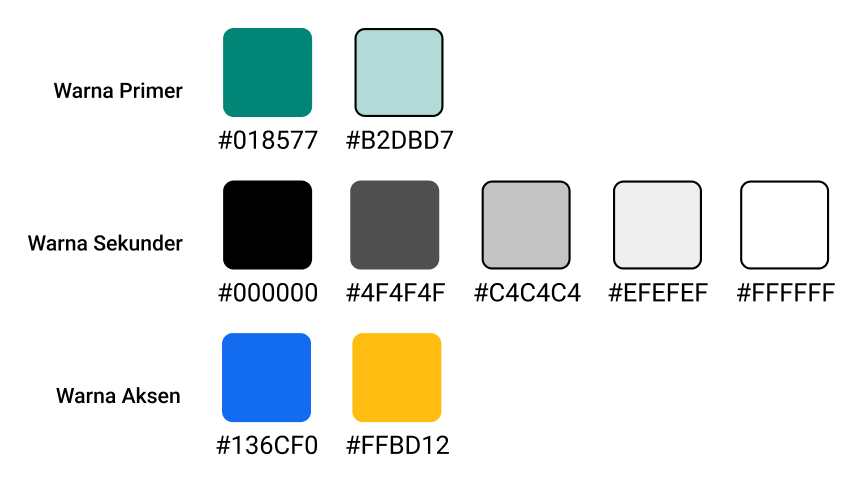
\includegraphics[width=0.7\textwidth]{chapter-4-color.png}
  \caption{Palet Warna Prototipe Aplikasi}
  \label{img:pallete}
\end{figure}
\FloatBarrier

\subsubsection{Tipografi}
\label{subsubsec:aspek_tipografi}
Tipografi dalam prototipe menggunakan \textit{typeface} Roboto, sesuai dengan \textit{typeface} yang digunakan oleh aplikasi Digital Wellbeing, dan merupakan \textit{typeface} standar yang digunakan dalam \textit{smartphone} berbasis Android. Tampilan dari \textit{typeface} Roboto dapat dilihat pada Gambar \ref{img:typeface}.

\begin{figure}[h]
  \centering
  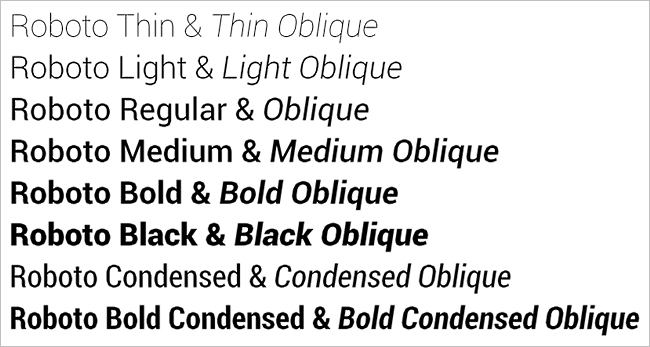
\includegraphics[width=0.6\textwidth]{chapter-4-roboto.jpg}
  \caption{\textit{Typeface} Roboto}
  \label{img:typeface}
\end{figure}
\FloatBarrier

\subsubsection{Ikon}
\label{subsubsec:aspek_ikon}
Ikon adalah simbol grafis yang dapat merepresentasikan sebuah fungsi atau objek pada antarmuka aplikasi. Penggunaan ikon yang sering ditemukan di tampilan aplikasi lain juga dapat memberikan rasa familiaritas, mempermudah fungsi-fungsi untuk dipelajari. Ikon-ikon yang digunakan pada prototipe \textit{high-fidelity} akan diambil dari ikon-ikon Material Design. Warna ikon akan mengikuti konteks dari antarmuka di sekelilingnya atau kondisi penggunaan tertentu, yaitu bisa menggunakan warna primer, sekunder, atau aksen. Ikon-ikon yang digunakan pada prototipe dapat ditemukan pada Gambar \ref{img:icons}

\begin{figure}[h]
  \centering
  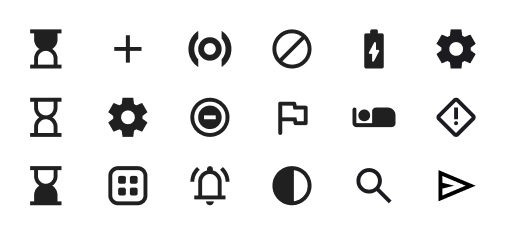
\includegraphics[width=0.5\textwidth]{chapter-4-icons.png}
  \caption{Ikon yang digunakan}
  \label{img:icons}
\end{figure}
\FloatBarrier
 
\subsubsection{Komponen Desain}
\label{subsubsec:aspek_komponen}

Berikut ini disebutkan beberapa komponen desain yang sering digunakan pada prototipe \textit{high-fidelity} Digital Wellbeing

\begin{enumerate}
  \item \textit{Button}
  \subitem Terdapat 3 jenis utama tombol pada prototipe, \textit{filled button}, \textit{border button}, dan \textit{text button}. Adapun variasi terhadap ukuran dan bentuk dari tombol yang diturunkan ketiga jenis utama. Tombol-tombol ini berperan penting dalam melakukan aksi dan menetapkan pengaturan. Beberapa tampilan memiliki deretan tombol-tombol jika terdapat lebih dari 1 aksi yang dapat dilakukan, maka dari itu desain yang berbeda dari tombol cukup penting untuk menegaskan hierarki kepentingan dari setiap aksi. Tampilan dari tombol-tombol yang digunakan dapat dilihat pada Gambar \ref{img:button}.
    \begin{figure}[h]
      \centering
      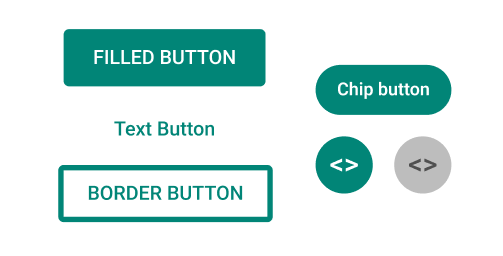
\includegraphics[width=0.45\textwidth]{chapter-4-buttons.png}
      \caption{Komponen \textit{button}}
      \label{img:button}
    \end{figure}
    \FloatBarrier
  
  \item Dialog
  \subitem Dialog adalah sebuah jendela kecil melayang yang digunakan untuk menampilkan secuplik informasi, meminta aksi dari pengguna, atau memuat pengaturan suatu fitur. Dialog sering dimanfaatkan pada prototipe untuk memuat pengaturan yang lebih kompleks atau informasi lebih di saat layar sudah cukup terpenuhi, berguna agar membebankan pengguna dengan tampilan yang terlalu rumit.

  \begin{figure}[h]
    \centering
    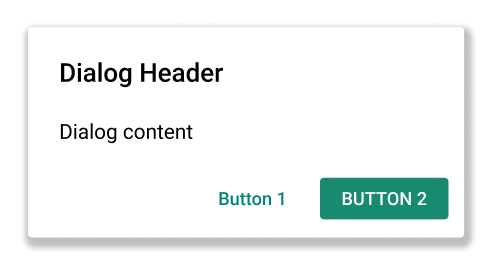
\includegraphics[width=0.4\textwidth]{chapter-4-dialog.png}
    \caption{Komponen dialog}
    \label{img:dialog}
  \end{figure}
  \FloatBarrier

  \item \textit{Time Picker}
  \subitem \textit{Time Picker} adalah sebuah variasi dari dialog yang berguna untuk memilih waktu. \textit{Time Picker} sering dimanfaatkan dalam prototipe, seperti untuk mengatur jadwal aktivasi Focus Mode atau App Timer.
  
  \begin{figure}[h]
    \centering
    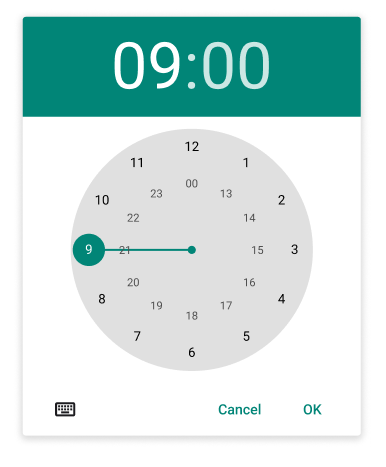
\includegraphics[width=0.35\textwidth]{chapter-4-timepicker.png}
    \caption{Komponen \textit{time picker}}
    \label{img:timepicker}
  \end{figure}
  \FloatBarrier

  \item \textit{Search bar}
  \subitem \textit{Search bar} adalah sebuah komponen untuk mencari sebuah benda dari dalam daftar. \textit{Search bar} sering dimanfaatkan pada prototipe karena banyaknya tampilan yang memuat daftar aplikasi, sehingga dibutuhkan untuk mempermudah pencarian aplikasi oleh pengguna.
 
  \begin{figure}[h]
    \centering
    
\includegraphics[width=0.6\textwidth]{chapter-4-seachbar.png}
    \caption{Komponen \textit{search bar}}
    \label{img:searchbar}
  \end{figure}
  \FloatBarrier

  \item \textit{Bar chart}
  \subitem \textit{Bar chart} atau diagram batang adalah sebuah grafik yang terusun dari kolom-kolom berbentuk batang. \textit{Bar chart} digunakan dalam prototipe untuk menyampaikan informasi tentang data penggunaan \textit{smartphone} atau aplikasi.
 
  \begin{figure}[h]
    \centering
    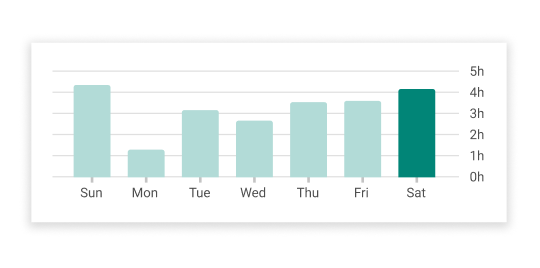
\includegraphics[width=0.5\textwidth]{chapter-4-barchart.png}
    \caption{Komponen \textit{bar chart}}
    \label{img:barchart}
  \end{figure}
  \FloatBarrier

  \item \textit{Dropdown}
  \subitem \textit{Dropdown} adalah sebuah komponen desain yang berguna untuk mengelompokkan dan menyembunyikan objek-objek dengan atribut yang serupa. Komponen \textit{dropdown} dimanfaatkan pada prototipe untuk mengumpulkan pengaturan yang mirip pada suatu halaman, dan berguna untuk mengurangi beban visual dari tammpilan layar. Komponen \textit{dropdown} juga sudah digunakan pada aplikasi Digital Wellbeing pada awalnya.
 
  \begin{figure}[h]
    \centering
    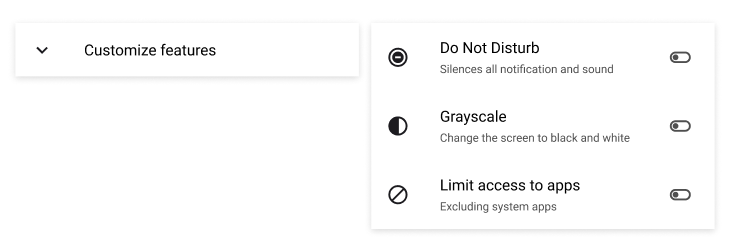
\includegraphics[width=0.6\textwidth]{chapter-4-dropdown.png}
    \caption{Komponen \textit{dropdown}}
    \label{img:dropdown}
  \end{figure}
  \FloatBarrier

\end{enumerate}


\subsection{Batasan Pengembangan}
\label{subsec:hifi_1_batasan}

Pengembangan prototipe \textit{high-fidelity} ini memiliki beberapa batasan agar pengembangan dapat fokus pada tujuan pengujian. Batasan-batasan pengembangan prototipe \textit{high-fidelity} adalah sebagai berikut

\begin{enumerate}
  \item Pengembangan prototipe \textit{high-fidelity} akan menggunakan kakas Figma.
  \item Data yang digunakan dalam prototipe berupa \textit{mock data} yang ditentukan oleh desainer.
  \item Prototipe dikembangkan untuk \textit{smartphone} berdimensi layar ukuran 360x800 pixel.
  \item Prototipe tidak mendukung kemampuan untuk input data kustom, bila komponen prototipe ditujukan untuk input data maka data yang ditunjukkan telah ditentukan oleh desainer.
  \item Tampilan prototipe menggunakan Bahasa Inggris. 
  \item Fitur rekomendasi pada prototipe tidak menggunakan rekomendasi nyata atas analisis data pengguna.
  \item Homescreen pada prototipe tidak mengacu pada tampilan \textit{smartphone} merk tertentu dengan alasan fokus pada tujuan untuk menguji komponen-komponen prototipe yang tidak dapat diakses dari dalam aplikasi.
\end{enumerate}

\subsection{Implementasi Prototipe \textit{High-Fidelity} Iterasi Pertama}
\label{subsec:hifi_1_implementasi}

% Berdasarkan rencana perbaikan pada Tabel \ref{tab:daftar_perbaikan_lofi}, analisis aspek antarmuka, dan batasan pengembangan, maka tampilan-tampilan prototipe \textit{low-fidelity} pada Tabel \ref{tab:daftar_lofi_halaman} dan Tabel \ref{tab:daftar_lofi_widget} akan dikembangkan dan diimplementasi menjadi prototipe \textit{high-fidelity}. Berikut adalah hasil implementasi prototipe \textit{high-fidelity} iterasi pertama.

% \begin{enumerate}
%   \item Main Menu
%   \subitem Halaman ini adalah tampilan utama dari aplikasi Digital Wellbeing yang memuat navigasi utama ke fitur-fitur lainnya. Pada prototipe \textit{high-fidelity} terdapat perubahan pada bentuk menu navigasi menjadi lebih bundar agar lebih \textit{user-friendly}. Adapun implementasi ilustrasi untuk menu Focus Mode dan Bedtime Mode, dan ikon-ikon pada menu lainnya, menggantikan \textit{placeholder} pada tampilan \textit{low-fidelity}.
  
%   \begin{figure}[h]
%     \centering
%     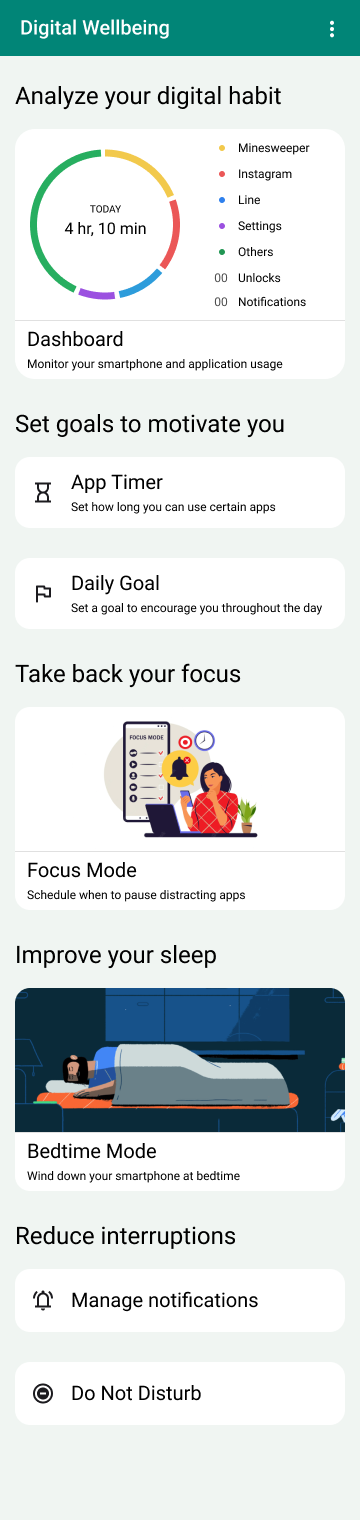
\includegraphics[width=0.3\textwidth]{hifi/h-01}
%     % \caption{Komponen \textit{dropdown}}
%     % \label{img:dropdown}
%   \end{figure}
%   \FloatBarrier



% \end{enumerate}

% Tabel \ref{tab:daftar_hifi_halaman} memuat implementasi tampilan halaman prototipe \textit{high-fidelity}, sedangkan Tabel \ref{tab:daftar_hifi_widget} memuat implementasi tampilan untuk \textit{widget}. Pada kedua tabel tersebut dimuat juga pemetaan prinsip desain tambahan terhadap prototipe \textit{high-fidelity}, serta penjelasan singkat tentang tampilan prototipe \textit{high-fidelity} dan perubahannya dari tampilan prototipe \textit{low-fidelity}.

Berdasarkan rencana perbaikan pada Tabel \ref{tab:daftar_perbaikan_lofi}, analisis aspek antarmuka, dan batasan pengembangan, maka tampilan-tampilan prototipe \textit{low-fidelity} pada Tabel \ref{tab:daftar_lofi_halaman} dan Tabel \ref{tab:daftar_lofi_widget} akan dikembangkan dan diimplementasi menjadi prototipe \textit{high-fidelity}. Tabel \ref{tab:daftar_hifi_halaman} memuat implementasi tampilan halaman prototipe \textit{high-fidelity}, sedangkan Tabel \ref{tab:daftar_hifi_widget} memuat implementasi tampilan untuk \textit{widget}. Pada kedua tabel tersebut dimuat juga pemetaan \textit{usability goals} dan \textit{user experience goals} yang ingin dicapai dari halaman prototipe \textit{high-fidelity}, serta penjelasan singkat tentang tampilan prototipe \textit{high-fidelity} dan perubahannya dari tampilan prototipe \textit{low-fidelity}.


\newlength{\hifiwidth}
\setlength{\hifiwidth}{0.315\textwidth}

\newlength{\hifidescwidth}
\setlength{\hifidescwidth}{0.315\textwidth}

\newcommand{\hifidesc}[1]{\desc{\hifidescwidth}{#1}}

\newcommand{\hifi}[1]{\begin{center}\includegraphics[width=\hifiwidth]{#1}\end{center}}
\newcommand{\hifiwidget}[2]{\begin{center}\includegraphics[width=#1]{#2}\end{center}}

\RaggedLeft
\begin{footnotesize}
\begin{longtable}[c]{|>{\ccnormspacingcenter}p{0.12\textwidth}|>{\ccnormspacing}p{\hifidescwidth}|>{\ccnormspacingcenter}p{0.12\textwidth}|>{\ccnormspacingcenter}p{\hifiwidth}|}
  \caption{Daftar Tampilan Halaman Prototipe \textit{High-Fidelity}}
  \label{tab:daftar_hifi_halaman} \\
  \hline \rowcolor[HTML]{A3E5F5}
  \centering\textbf{Halaman} & \centering\textbf{Penjelasan Halaman} & \centering\textbf{\textit{Goals}} & \textbf{Prototipe \textit{High-Fidelity}} \\ \hline \endfirsthead
  
  % \caption*{\autoref{tab:daftar_hifi_halaman} (lanjutan): Daftar Tampilan Halaman Prototipe \textit{High-Fidelity}} \\
  \hline \rowcolor[HTML]{A3E5F5}
  \centering\textbf{Halaman} & \centering\textbf{Penjelasan Halaman} & \centering\textbf{\textit{Goals}} & \textbf{Prototipe \textit{High-Fidelity}} \\ \hline \endhead
  \hline \endfoot

  \textbf{H-01} Halaman Main Menu & 
    \hifidesc{
      Halaman ini adalah tampilan utama dari aplikasi Digital Wellbeing yang memuat navigasi utama ke fitur-fitur lainnya. Pada prototipe \textit{high-fidelity} terdapat perubahan pada bentuk menu navigasi menjadi lebih bundar agar lebih \textit{user-friendly}. Adapun implementasi ilustrasi untuk menu Focus Mode dan Bedtime Mode, dan ikon-ikon pada menu lainnya, menggantikan \textit{placeholder} pada tampilan \textit{low-fidelity}.
    } & G-02, G-04 & \hifi{hifi/h-01} \\ \hline
  
  \textbf{H-02} Halaman Dashboard &
    \hifidesc{
      Halaman ini memuat seluruh data penggunaan \textit{smartphone}. Pada prototipe \textit{high-fidelity} terdapat penambahan warna untuk \textit{bar chart} agar memperjelas data yang sedang dipilih. \newline 
      Adapun pengubahan desain dari tombol penambahan App Group untuk memberikan perbedaan yang jelas dengan tombol navigasi ke halaman data penggunaan App Group
    }
  & G-01, G-02, G-03, G-04 & \hifi{hifi/h-02} \\ \hline
  
  \textbf{H-03} Halaman App Timer & 
    \hifidesc{
      Halaman ini berisi daftar App Timer yang telah dipasang oleh pengguna, dan daftar aplikasi lain. Pada prototipe \textit{high-fidelity}, menu konfigurasi pengingat App Timer disembunyikan di dalam komponen \textit{dropdown} untuk mengurangi kompleksitas visual. Selain itu, ada juga penambahan bagian yang memuat daftar App Group yang sudah dibuat, memindahkan lokasi App Group dari dalam daftar aplikasi.
    } & G-01, G-03 & \hifi{hifi/h-03} \\ \hline
  
  \textbf{H-04} Halaman Daily Goal & 
    \hifidesc{
      Di halaman ini, pengguna dapat menentukan Daily Goal atau tujuan harian yang ingin ditempuh dan dibantu diingatkan oleh aplikasi Digital Wellbeing. Pada prototipe \textit{high-fidelity} terdapat penambahan penjelasan untuk fitur-fitur pengingat Daily Goal agar lebih mudah untuk dimengerti. Adapun penambahan ikon untuk fitur Daily Goal agar tampilan tidak terasa kaku
    } & G-04 & \hifi{hifi/h-04} \\ \hline
  
  \textbf{H-05} Halaman Focus Mode & 
    \hifidesc{
      Halaman ini memuat status dari keberjalanan Focus Mode serta aksi-aksi yang dapat dilakukan untuk menunda, mematikan, atau mengaktivasinya. Pada prototipe \textit{high-fidelity} terdapat penambahan daftar aplikasi untuk memilih aplikasi yang dinilai mendistraksi, daftar ini dapat dimanfaatkan jika pengguna ingin menyalakan fitur Focus Mode tanpa mengikuti jadwal. Adapun pemindahan lokasi navigasi ke halaman penambahan jadwal Focus Mode agar lebih mudah diakses jika terdapat banyak jadwal Focus Mode.
     } & G-01, G-03 & \hifi{hifi/h-05} \\ \hline
  
  \textbf{H-06} Halaman Bedtime Mode &  
    \hifidesc{
      Pada halaman ini, pengguna dapat mengatur jadwal aktivasi Bedtime Mode menurut mode perilaku aktivasi yang dipilihnya. Pada prototipe \textit{high-fidelity} terdapat penambahan penjelasan singkat tentang mode aktivasi While Charging, sesuai dengan rencana perbaikan terhadap masalah yang dilaporkan. Adapun penambahan warna aksen terhadap pengaturan jadwal, warna aksen ini sudah menjadi bagian dari aplikasi Digital Wellbeing pada awalnya. Selain itu, menu konfigurasi kemampuan yang aktif saat Bedtime Mode disembunyikan di dalam komponen \textit{dropdown} untuk mengurangi kompleksitas visual.
    } & G-03 & \hifi{hifi/h-06-schedule} \\ \hline
  
  \textbf{H-07} Halaman Ringkasan Penggunaan Aplikasi & 
    \hifidesc{
      Halaman ini memuat data penggunaan sebuah aplikasi. Pada prototipe \textit{high-fidelity}, terdapat penambahan ikon pada navigasi App Timer dan pengaturan notifikasi agar tampilan lebih mudah dikenali.
    } & G-03 & \hifi{hifi/h-07} \\ \hline
  
  \textbf{H-08} Halaman Ringkasan Penggunaan App Group & 
    \hifidesc{
      Halaman ini memuat data penggunaan dari App Group atau kelompok aplikasi yang ditentukan oleh pengguna. Pada prototipe \textit{high-fidelity}, terdapat penambahan ikon pada navigasi App Timer dan pengaturan App Group agar tampilan lebih mudah dikenali.
    } & G-01, G-03 & \hifi{hifi/h-08} \\ \hline
  
  \textbf{H-09} Halaman Pengaturan App Group & 
    \hifidesc{
      Pada halaman ini dapat dilakukan pengaturan terhadap App Group yang dibuat oleh pengguna. Pada prototipe \textit{high-fidelity}, tidak ada perubahan yang cukup signifikan selain pengaplikasian warna.
    } & G-01, G-03 & \hifi{hifi/h-09} \\ \hline
  
  \textbf{H-10} Halaman Pengaturan Jadwal App Timer & 
    \hifidesc{
      Pada halaman ini dapat dilakukan pengaturan terhadap App Timer aplikasi yang dibuat oleh pengguna. Pada prototipe \textit{high-fidelity} terdapat perubahan tampilan untuk pengaturan App Timer, dengan memberikan elemen untuk mengkonfirmasi pengaturan sesuai dengan rancangan perbaikan dari prototipe \textit{low-fidelity}. \newline
      Adapun tambahan jika belum ada opsi mode aktivasi App Timer, maka tombol konfirmasi pengaturan akan dinonaktifkan, mengikuti prinsip desain \textit{Constraint} (DP-07).
    } & G-01, G-03 & \hifi{hifi/h-10-daily} \hifi{hifi/h-10-off} \\ \hline
  
  \textbf{H-11} Halaman Pengaturan Jadwal Focus Mode & 
    \hifidesc{
      Pada halaman ini, pengguna dapat mengatur hari dan waktu aktivasi dari jadwal Focus Mode yang dibuat pengguna. Pada prototipe \textit{high-fidelity} terdapat penambahan bagian yang memuat daftar App Group yang sudah dibuat, memindahkan lokasi App Group dari dalam daftar aplikasi, agar pengguna lebih mudah dalam memilih sekelompok aplikasi sekaligus.
    } & G-01, G-03 & \hifi{hifi/h-11} \\ \hline
  
  \textbf{H-12} Halaman Pengenalan Dashboard & 
    \hifidesc{
      Halaman ini memuat ilustrasi tujuan dari Dashboard dan penjelasan tentang fitur-fitur yang terdapat pada Dashboard. Pada prototipe \textit{high-fidelity} dilakukan perubahan ukuran \textit{font} dari deskripsi agar lebih mudah dibaca. Adapun penambahan ilustrasi agar fitur-fitur yang dijelaskan lebih mudah untuk dipelajari.
    } & G-02 & \hifi{hifi/h-12} \\ \hline
  
  \textbf{H-13} Halaman Pengenalan App Timer & 
    \hifidesc{
      Halaman ini memuat ilustrasi tujuan dari App Timer dan penjelasan tentang fitur-fitur yang terdapat pada App Timer. Pada prototipe \textit{high-fidelity} dilakukan perubahan ukuran \textit{font} dari deskripsi agar lebih mudah dibaca. Adapun penambahan ilustrasi agar fitur-fitur yang dijelaskan lebih mudah untuk dipelajari.
    } & G-02 & \hifi{hifi/h-13} \\ \hline
  
  \textbf{H-14} Halaman Pengenalan Goal Reminder & 
    \hifidesc{
      Halaman ini memuat ilustrasi tujuan dari Goal Reminder dan penjelasan tentang fitur-fitur yang terdapat pada Goal Reminder. Pada prototipe \textit{high-fidelity} dilakukan perubahan ukuran \textit{font} dari deskripsi agar lebih mudah dibaca. Adapun penambahan ilustrasi agar fitur-fitur yang dijelaskan lebih mudah untuk dipelajari.
    } & G-02 & \hifi{hifi/h-14} \\ \hline
  
  \textbf{H-15} Halaman Pengenalan Focus Mode & 
    \hifidesc{
      Halaman ini memuat ilustrasi tujuan dari Focus Mode dan penjelasan tentang fitur-fitur yang terdapat pada Focus Mode. Pada prototipe \textit{high-fidelity} dilakukan perubahan ukuran \textit{font} dari deskripsi agar lebih mudah dibaca. Adapun penambahan ilustrasi agar fitur-fitur yang dijelaskan lebih mudah untuk dipelajari.
    } & G-02 & \hifi{hifi/h-15} \\ \hline
  
  \textbf{H-16} Halaman Pengenalan Bedtime Mode & 
    \hifidesc{
      Halaman ini memuat ilustrasi tujuan dari Bedtime Mode dan penjelasan tentang fitur-fitur yang terdapat pada Bedtime Mode. Pada prototipe \textit{high-fidelity} dilakukan perubahan ukuran \textit{font} dari deskripsi agar lebih mudah dibaca. Adapun penambahan ilustrasi agar fitur-fitur yang dijelaskan lebih mudah untuk dipelajari.
    } & G-02 & \hifi{hifi/h-16} \\ \hline

\end{longtable}
\end{footnotesize}
\justifying
\FloatBarrier

\RaggedLeft
\begin{footnotesize}
\begin{longtable}[c]{|>{\ccnormspacingcenter}p{0.12\textwidth}|>{\ccnormspacing}p{\hifidescwidth}|>{\ccnormspacingcenter}p{0.12\textwidth}|>{\ccnormspacingcenter}p{\lofiwidth}|}
  \caption{Daftar Tampilan \textit{Widget} Prototipe \textit{High-Fidelity}}
  \label{tab:daftar_hifi_widget} \\
  \hline \rowcolor[HTML]{A3E5F5}
  \centering\textbf{ID \textit{Widget}} & \centering\textbf{Penjelasan \textit{Widget}} & \centering\textbf{Goals} & \textbf{Prototipe \textit{Low-Fidelity}} \\ \hline \endfirsthead
  \hline \rowcolor[HTML]{A3E5F5}
  \centering\textbf{ID \textit{Widget}} & \centering\textbf{Penjelasan \textit{Widget}} & \centering\textbf{Goals} & \textbf{Prototipe \textit{Low-Fidelity}} \\ \hline \endhead
  \hline \endfoot
  
  \textbf{W-01} \textit{Widget} Dashboard & 
    \hifidesc{
      \textit{Widget} ini memuat data penggunaan \textit{smartphone}, serta 3 aplikasi dengan penggunaan tertinggi pada hari tersebut. Desain \textit{widget} pada prototipe \textit{high-fidelity} dibuat menjadi lebih \textit{user-friendly} agar \textit{widget} dapat lebih berbaur dengan tampilan pada Homescreen.
    } & G-01, G-03, G-04 & \hifiwidget{0.2\textwidth}{hifi/w-01} \\ \hline

  \textbf{W-02} \textit{Widget} App Timer & 
    \hifidesc{
      \textit{Widget} ini memuat daftar aplikasi yang telah dipasang App Timer, serta sisa waktu untuk menggunakan aplikasi sebelum aksesnya ditutup. Desain \textit{widget} pada prototipe \textit{high-fidelity} dibuat menjadi lebih \textit{user-friendly} agar \textit{widget} dapat lebih berbaur dengan tampilan pada Homescreen.
    } & G-01, G-03, G-04 & \hifiwidget{0.325\textwidth}{hifi/w-02} \\ \hline
  
  \textbf{W-03} \textit{Widget} Focus Mode & 
    \hifidesc{
      \textit{Widget} ini menampilkan status keberlangsungan dari Focus Mode. Desain \textit{widget} pada prototipe \textit{high-fidelity} dibuat menjadi lebih \textit{user-friendly} agar \textit{widget} dapat lebih berbaur dengan tampilan pada Homescreen. Ada juga penambahan interaksi pada \textit{widget} agar pengguna dapat memanfaatkan lebih banyak fungsionalitas dari Focus Mode.
    } & G-01, G-03, G-04 & \hifiwidget{0.325\textwidth}{hifi/w-03} \\ \hline

\end{longtable}
\end{footnotesize}
\justifying
\FloatBarrier


% \subsection{Kaitan \textit{Usability Goals} dan \textit{User Experience Goals} dengan Prototipe \textit{High-Fidelity}}




% * =======================================================================
% *   ||  ||  ||  ||  ||  ||  ||  ||  ||  ||  ||  ||  ||  ||  ||  ||  ||
% * =======================================================================

\section{Pengujian Prototipe \textit{High-Fidelity} Iterasi Pertama}
\label{sec:test_1}

Prototipe \textit{high-Fidelity} yang sudah dirancang perlu dilakukan pengujian. Pengujian dilakukan dengan menggunakan metode \textit{usability testing}. Pengujian prototipe \textit{low-fidelity} dilakukan untuk mengukur capaian dari tujuan-tujuan yang sudah ditentukan pada subbab \ref{subsec:analisis_goals}, yaitu \textit{usability goals} \textit{efficiency} dan \textit{learnability} serta \textit{user experience goals} \textit{helpful} dan \textit{motivating}. Untuk mengukur capaian-capaian tersebut, partisipan diminta untuk menyelesaikan beberapa \textit{task} terkait halaman, widget, dan fitur yang telah dirancang. Pada Tabel \ref{tab:daftar_pengujian_goals}, dilakukan pemetaan \textit{usability goals} dan \textit{user experience goals} dengan tujuan dan kriteria pengujian yang berkaitan.

\RaggedLeft
\begin{small}
\begin{longtable}[c]{|W{c}{0.16\textwidth}|>{\ccnormspacing}m{0.36\textwidth}|>{\ccnormspacing}m{0.36\textwidth}|}
  \caption{Pemetaan Tujuan dan Kriteria Pengujian terhadap \textit{Usability} dan \textit{User Experience Goals}}
  \label{tab:daftar_pengujian_goals} \\
  \hline \rowcolor[HTML]{A3E5F5}
  \textbf{Goals} & \multicolumn{1}{|c|}{\textbf{Tujuan Pengujian}} & \multicolumn{1}{|c|}{\textbf{Kriteria Pengujian}} \\ \hline \endfirsthead
  \hline \rowcolor[HTML]{A3E5F5}
  \textbf{Goals} & \multicolumn{1}{|c|}{\textbf{Tujuan Pengujian}} & \multicolumn{1}{|c|}{\textbf{Kriteria Pengujian}}\\ \hline \endhead
  \hline \endfoot

  % Usability Goals
  % \textit{Efficiency} & Mengukur seberapa efisien pengguna dalam melakukan aktivitasnya di dalam prototipe \textit{high-fidelity} & Mengukur waktu yang diperlukan dalam mengerjakan setiap \textit{task}, dan menggunakan kuesioner dari \textit{System Usability Scale} \\ \hline
  \textit{Efficiency} & Mengukur seberapa efisien pengguna dalam melakukan aktivitasnya di dalam prototipe \textit{high-fidelity} & Mengukur tingkat \textit{efficiency} aplikasi menggunakan kuesioner dari \textit{System Usability Scale} \\ \hline
  
  \textit{Learnability} & Mengukur seberapa mudah fitur-fitur aplikasi untuk dipelajari dan digunakan oleh pengguna & Mengukur tingkat kemudahan penggunaan aplikasi dengan \textit{Single Ease Question}\\ \hline
  
  % UX Goals
  \textit{Helpful} & Mengetahui apakah pengguna dapat merasa terbantu dalam melakukan aktivitasnya oleh fitur-fitur yang disediakan prototipe \textit{high-fidelity}  & Menggunakan skala \textit{value/usefulness} dari \textit{Intrinsic Motivation Inventory} untuk mengukur seberapa membantu aplikasi kepada pengguna \\ \hline
  
  \textit{Motivating} & Mengetahui apakah pengguna dapat merasa termotivasi untuk fokus pada pekerjaannya oleh fitur-fitur yang disediakan prototipe \textit{high-fidelity} & Menggunakan skala \textit{interest/enjoyment}, dan \textit{pressure/tension} dari \textit{Intrinsic Motivation Inventory} untuk mengukur tingkat motivasi pengguna setelah melakukan pengujian \\ \hline

\end{longtable}
\end{small}
\justifying
\FloatBarrier

\subsection{Langkah Pengujian}
\label{subsec:test_1_langkah}

Pengujian dilakukan dengan beberapa tahap, yaitu perkenalan, eksplorasi, pengerjaan \textit{task}, lalu diakhiri dengan penutupan. Rancangan pengujian yang lebih detail dapat dilihat pada Lampiran \ref{chpt:testing_hifi}. Berikut adalah penjelasan untuk setiap tahap pengujian

\begin{enumerate}
  \item Perkenalan
  \subitem Pada tahap ini, dilakukan perkenalan diri serta pengarahan singkat kepada partisipan. Pengarahan akan berisi pemaparan tentang prototipe yang akan diuji serta penjelasan terkait prosedur pengujian. 

  \item Eksplorasi
  \subitem Pada tahap ini, partisipan diberi kesempatan untuk melakukan eksplorasi terhadap prototipe yang akan diuji. Hal ini bertujuan agar partisipan memiliki wawasan yang cukup tentang aplikasi sebelum pengujian.

  \item Pengerjaan \textit{task}
  \subitem Pada tahap ini, partisipan mulai mengerjakan \textit{task-task} yang diberikan. Detail lebih lengkap dari task dapat dilihat pada Lampiran \ref{chpt:skenario_hifi1}. Setiap mengerjakan \textit{task}, kegiatan partisipan akan direkam waktunya sebagai bagian dari pengujian \textit{usability goal efficiency}. Selain itu, setiap kali partisipan selesai mengerjakan sebuah \textit{task}, mereka diminta untuk mengisi \textit{post-task questionnaire} yaitu \textit{Single Ease Question} (SEQ). SEQ menggunakan pertanyaan dengan jawaban \textit{likert-scale} untuk mengukur tingkat kemudahan penggunaan fitur dalam aplikasi.

  \item Pengisian \textit{post-test questionnaire}
  \subitem Pada tahap ini, partisipan telah selesai mengerjakan seluruh \textit{task} yang diberikan penguji. Partisipan akan diminta untuk mengisi \textit{post-test questionnaire} dalam bentuk \textit{System Usability Scale} (SUS) dan \textit{Intrinsic Motivation Inventory} (IMI). 

  \item Penutupan
  \subitem Pada tahap ini, pengujian diakhiri dengan penyampaian kesan pesan dari partisipan, serta ucapan terima kasih dari penguji. 

\end{enumerate}


\subsection{Hasil Pengujian Prototipe \textit{High-Fidelity} Iterasi Pertama}
\label{subsec:test_1_hasil}

Pengujian prototipe \textit{high-fidelity} iterasi pertama dilakukan dengan 5 (lima) orang, sesuai dengan perkataan dari \textcite{nielsenusabilityproblems} yang menyebutkan bahwa pengujian dengan 5 (lima) orang partisipan sudah cukup untuk menemukan rata-rata 85\% masalah dari desain, dalam hal ini prototipe \textit{high-fidelity}. Hasil pengujian lengkap dapat dilihat pada Lampiran \ref{chpt:hasil_test_hifi1}. Dari pengujian, didapatkan beberapa temuan penting dari partisipan tentang prototipe, yang rangkumannya dapat dilihat pada Tabel \ref{tab:daftar_temuan_hifi}


\RaggedLeft
\begin{footnotesize}
\begin{longtable}[c]{|W{c}{0.12\textwidth}|>{\ccnormspacingcenter}m{0.8\textwidth}|}
  \caption{Daftar Temuan Penting Pengujian Prototipe \textit{High-Fidelity} Iterasi Pertama}
  \label{tab:daftar_temuan_hifi} \\
  \hline \rowcolor[HTML]{A3E5F5}
  \textbf{Partisipan} & \textbf{Temuan Penting} \\ \hline \endfirsthead
  \hline \rowcolor[HTML]{A3E5F5}
  \textbf{Partisipan} & \textbf{Temuan Penting} \\ \hline \endhead
  \hline \endfoot

  1 & \cditem{
    \item Partisipan berekspektasi diberikan pengaturan \textit{default} Bedtime Mode berupa opsi jadwal
  } \\ \hline
    
  2 & \cditem{
    \item Partisipan merasa widget Dashboard memuat lebih dari 3 aplikasi teratas
    \item Partisipan merasa penjelasan pada halaman-halaman pengenalan fitur masih terlalu panjang
    } \\ \hline
    
  3 & \cditem{
    \item Partisipan merasa navigasi dari halaman Dashboard langsung ke App Timer tidak diperlukan dan cukup sulit dibedakan dengan navigasi ke halaman penggunaan aplikasi
  } \\ \hline
  
  4 & \cditem{
    \item Partisipan merasa memerlukan sebuah pesan pengingat sebelum mematikan Focus Mode atau App Timer untuk hari ini
    \item Partisipan merasa evaluasi Daily Goal sebaiknya tidak langsung muncul ketika selesai menentukan Daily Goal
  } \\ \hline
  
  5 & \cditem{
    \item Partisipan merasa penempatan fitur Smartphone Usage Evaluation kurang tepat pada halaman Daily Goal
    \item Partisipan merasa tombol + (plus) pada widget App Timer tidak diperlukan
  } \\ \hline

\end{longtable}
\end{footnotesize}
\justifying
\FloatBarrier

Berdasarkan temuan-temuan yang telah disebutkan di atas, maka disusun beberapa rencana perbaikan untuk direalisasikan dalam prototipe \textit{high-fidelity} iterasi kedua. Pada Tabel \ref{tab:daftar_perbaikan_hifi} dapat ditemukan daftar masalah yang disimpulkan dari temuan-temuan penting, beserta rencana perbaikan yang berkaitan.

\RaggedLeft
\begin{footnotesize}
  \begin{longtable}[c]{|W{c}{0.06\textwidth}|>{\ccnormspacing}m{0.32\textwidth}|>{\ccnormspacing}m{0.35\textwidth}|>{\ccnormspacingcenter}m{0.14\textwidth}|}  \caption{Daftar Rencana Perbaikan Prototipe \textit{High-Fidelity} Iterasi Pertama}
  \label{tab:daftar_perbaikan_hifi} \\
  \hline \rowcolor[HTML]{A3E5F5}
  \textbf{ID} & \centering\textbf{Kesimpulan Masalah dari Temuan} & \centering\textbf{Rencana Perbaikan} & \textbf{Keterkaitan} \\ \hline \endfirsthead
  \hline \rowcolor[HTML]{A3E5F5}
  \textbf{ID} & \centering\textbf{Kesimpulan Masalah dari Temuan} & \centering\textbf{Rencana Perbaikan} & \textbf{Keterkaitan} \\ \hline \endhead
  \hline \endfoot

  PH-01 & Kurangnya opsi \textit{default} sebagai rekomendasi bagi pengguna untuk Bedtime Mode & Mengatur opsi \textit{default} pada Bedtime Mode menjadi Based on schedule & DP-01 \\ \hline
  PH-02 & Kurangnya fungsionalitas dari widget Dashboard & Hal ini merupakan pilihan desain yang disengaja untuk mempertahankan kesederhanaan dari sebuah widget & G-01 \\ \hline
  PH-03 & Adanya navigasi ke halaman App Timer dari halaman Dashboard mengganggu navigasi ke halaman penggunaan aplikasi & Menghapus navigasi dari halaman Dashboard ke halaman App Timer, tanpa menghapus indikator App Timer & G-03, G-04 \\ \hline
  PH-04 & Kurangnya elemen yang menjaga pengguna dari kesalahan aksi pada fungsi yang cukup kritis & Menambahkan pesan pengingat untuk aksi yang cukup kritis seperti mematikan Focus Mode atau App Timer & DP-07 \\ \hline
  PH-05 & Kurangnya penundaan waktu untuk memunculkan evaluasi dari penentuan Daily Goal  & Menunda memunculkan evaluasi tepat setelah menentukan Daily Goal & DP-06 \\ \hline
  PH-06 & Kurang tepatnya penempatan fitur Smartphone Usage Evaluation pada halaman Daily Goal & Memindahkan fitur Smartphone Usage Evaluation dari halaman Daily Goal ke halaman baru & G-01, G-02, G-04 \\ \hline
  PH-07 & Tidak diperlukannya tombol penambahan App Timer untuk widget App Timer & Menghapus tombol penambahan App Timer dari widget App Timer & G-01, G-03 \\ \hline
  
\end{longtable}
\end{footnotesize}
\justifying
\FloatBarrier

\newpage

\subsection{Analisis Hasil Pengujian Prototipe \textit{High-Fidelity} Iterasi Pertama}
\label{subsec:test_1_analisis}

Dari hasil pengujian pada prototipe \textit{high-fidelity} iterasi pertama, didapatkan beberapa skor dan temuan penting dari pengguna menurut kriteria-kriteria pengujian yang telah disebutkan pada Tabel \ref{tab:daftar_pengujian_goals}. Berikut adalah beberapa penjelasannya

\begin{enumerate}
  \item \textit{Single Ease Question} (SEQ)
  \subitem  Penilaian SEQ digunakan untuk mengetahui tingkat kemudahan sebuah \textit{task} untuk dapat diselesaikan oleh partisipan. Berdasarkan hasil nilai SEQ yang terdapat pada Gambar \ref{img:seq_1}, terlihat bahwa nilai yang diberikan setiap partisipan terhadap kemudahan pengerjaan setiap task sudah cukup baik, dengan nilai rata-rata terendah sebesar 5.7 pada \textit{task} 7. Oleh karena itu, aplikasi dinilai memiliki \textit{learnability} yang cukup baik. 

  \begin{figure}[h]
    \centering
    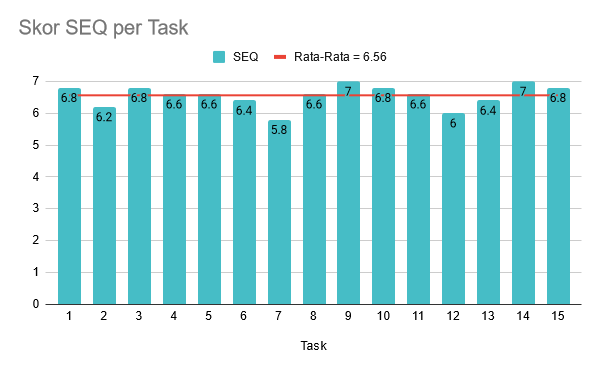
\includegraphics[width=0.6\textwidth]{hifi/hasil-seq.png}
    \caption{Hasil \textit{Single Ease Question} Pengujian Prototipe \textit{High-Fidelity} Iterasi Pertama}
    \label{img:seq_1}
  \end{figure}
  \FloatBarrier

  \item \textit{System Usability Scale} (SUS)
  \subitem  Berdasarkan hasil nilai SUS yang tertera pada Gambar \ref{img:sus_1} terlihat bahwa nilai yang diberikan setiap partisipan pada pengerjaan setiap \textit{task} sudah baik. Namun ditemukan bahwa nilai rata-rata SUS terendah adalah 65. Maka dari itu, desain solusi aplikasi masih perlu diperbaiki dalam prototipe \textit{high-fidelity} iterasi kedua agar dapat mencapai \textit{usability goal efficiency} dengan lebih baik. 

  \begin{figure}[h]
    \centering
    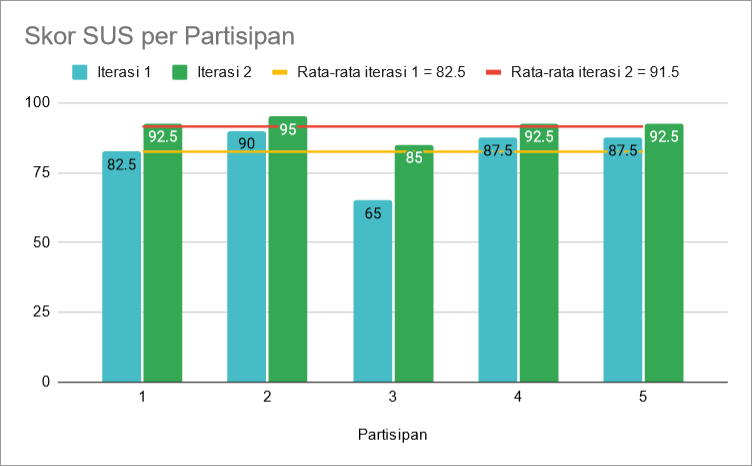
\includegraphics[width=0.6\textwidth]{hifi/hasil-sus.png}
    \caption{Hasil \textit{System Usability Scale} Pengujian Prototipe \textit{High-Fidelity} Iterasi Pertama}
    \label{img:sus_1}
  \end{figure}
  \FloatBarrier

  \item \textit{Intrinsic Motivation Inventory} (IMI)
  \subitem  Berdasarkan Gambar \ref{img:imi1_1} dapat dilihat bahwa skor IMI untuk sub skala \textit{Value/Usefulness} yang didapatkan dari setiap partisipan telah melewati nilai 5 dengan rata-rata skor 6,46. Dengan demikian, rancangan prototipe \textit{high-fidelity} sudah mengarah kepada \textit{user experience goal helpful} dengan baik, namun tetap dibutuhkan beberapa perbaikan yang perlu diperhatikan kembali.
  
  \begin{figure}[h]
    \centering
    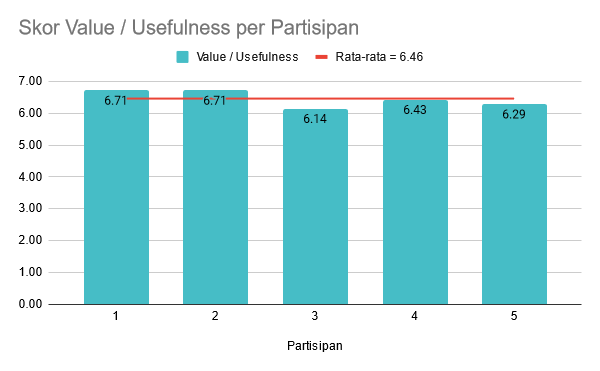
\includegraphics[width=0.6\textwidth]{hifi/hasil-imi1.png}
    \caption{Hasil \textit{Intrinsic Motivation Inventory} Sub Skala \textit{Value/Usefulness} Pengujian Prototipe \textit{High-Fidelity} Iterasi Pertama}
    \label{img:imi1_1}
  \end{figure}
  \FloatBarrier
  
  \subitem  Berdasarkan Gambar \ref{img:imi2_1} dapat dilihat bahwa skor IMI untuk sub skala \textit{Interest/Enjoyment} yang didapatkan dari setiap partisipan telah melewati nilai 5 dengan rata-rata skor 5,69. Di sisi lain, skor IMI untuk sub skala \textit{Pressure/Tension} memiliki nilai rata-rata setelah di-\textit{reverse} yaitu 6,52, yang telah melewati nilai batas 5 juga. Hal tersebut menunjukkan bahwa rancangan prototipe \textit{high-fidelity} sudah cukup mengarah kepada \textit{user experience goal motivating}, dengen perlu perbaikan yang cukup signifikan.

  \begin{figure}[h]
    \centering
    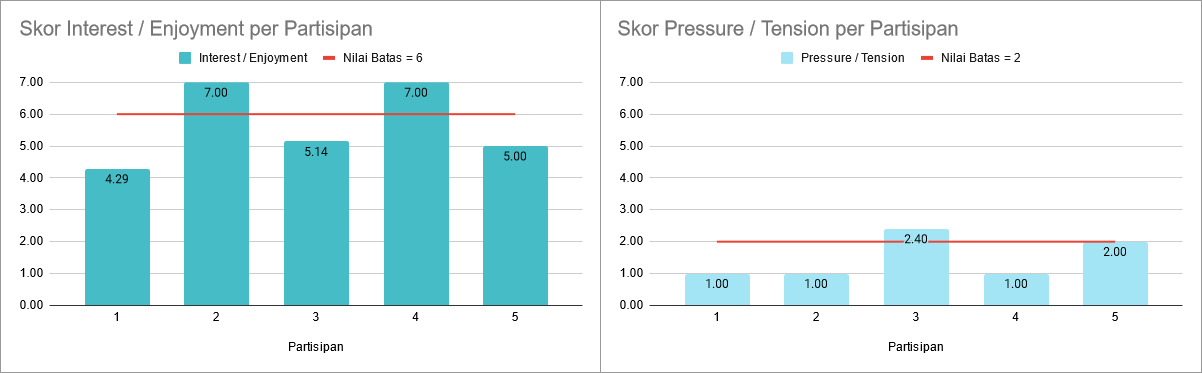
\includegraphics[width=0.9\textwidth]{hifi/hasil-imi2.png}
    \caption{Hasil \textit{Intrinsic Motivation Inventory} Sub Skala \textit{Interest/Enjoyment} dan \textit{Pressure/Tension} Pengujian Prototipe \textit{High-Fidelity} Iterasi Pertama}
    \label{img:imi2_1}
  \end{figure}
  \FloatBarrier

\end{enumerate}





